\documentclass[a4paper,11pt]{article}

%%%%%%%%%
%%usees%%
%%%%%%%%%
\usepackage[utf8]{inputenc}
%\usepackage[ngerman]{babel}
%\usepackage{a4wide}
\usepackage[margin=3.0cm, top=3.0cm, bottom=3.0cm]{geometry}
\usepackage{setspace}
\usepackage{graphicx}
\usepackage{amssymb} 
\usepackage{amsmath}
\usepackage{mathtools}
\usepackage{footnote}
\usepackage{caption}
\usepackage{color}
\usepackage[hidelinks]{hyperref}
\usepackage{cite}
\usepackage{todonotes}
\usepackage{subfigure}
\usepackage{siunitx}
\usepackage{tabularx}
\usepackage{wrapfig}
\usepackage{url}
\usepackage{listings}


\newcommand{\reffig}[1]{Figure~\ref{#1}}
\newcommand{\refsec}[1]{Section~\ref{#1}}
\newcommand{\refdef}[1]{Definition~\ref{#1}}
\newcommand{\reflst}[1]{Listing~\ref{#1}}
\newcommand{\reftab}[1]{Table~\ref{#1}}

\definecolor{Mulberry}{cmyk}{0.34,0.90,0,0.02}
\definecolor{BrickRed}{cmyk}{0,0.89,0.94,0.28}
\lstset{language=C++,frame=none, basicstyle=\tt}
\lstdefinelanguage{CLIPS}{
  keywordsprefix=?,
  %keywordsprefix=\$,
  alsoletter={?=-<>*\$},
  keywordstyle=\color{Mulberry!80!black}\bfseries,
  keywords=[2]{deffunction, deftemplate, defrule, deffacts, defgeneric,
    defmodule, defadvice, defglobal, defmethod, definstance, defclass},
  keywordstyle=[2]\color{BrickRed!70!blue}\bfseries,
  keywords=[3]{slot, multislot, type, default, default-dynamic,
                      extends, crlf, range, nil, if, then, else, while,
                      not, or, switch, case, and, reset,
                      assert, test, declare, salience, return, bind, modify,
                      retract, explicit, unique, node-index-hash,
                      halt, printout, =>, <-},
  keywordstyle=[3]\color{darkgray}\bfseries,
  keywords=[4]{subsetp,progn, progn$, not, node-index-hash, create$,
    append$, length$, printout},%
  keywordstyle=[4]\color{gray}\bfseries,
  %identifierstyle=\color{black},
  sensitive=false,
  comment=[l]{;},
  commentstyle=\color{purple}\ttfamily,
  stringstyle=\color{red}\ttfamily,
  morestring=[b]"
}


\lstdefinestyle{CLIPS}
{
  language=CLIPS,
  basicstyle=\footnotesize\ttfamily\vspace{0.2cm},
  breaklines=true,
  showstringspaces=false,
  %keywordstyle=\bfseries,
  %keywordstyle=\color{Mulberry},
  frame=lines,
  belowcaptionskip=-3pt,
  emphstyle=\itshape,
  numbers=left,
  stepnumber=1,
  backgroundcolor=\color{gray!10},
  rulecolor=\color{gray!80},
  fillcolor=\color{gray!10},
  framexleftmargin=16pt,
  xleftmargin=16pt,
  %stringstyle=\color{BitterSweet},
  stringstyle=\color{BrickRed},
  commentstyle=\color{BrickRed},
  escapechar=\%,
  % emph={getup, servo, depends_skills},
  %emphstyle=\underbar,
  %numbers=left,
  %stepnumber=1,
  %%stringstyle=\ttfamily, % typewriter type for strings
  %float,
  captionpos=b
}

\lstdefinestyle{SmallCLIPS}{
  style=CLIPS,
  basicstyle=\ttfamily\footnotesize,
  numbersep=6pt,
}
\lstdefinestyle{ReallySmallCLIPS}{
  style=CLIPS,
  basicstyle=\ttfamily\scriptsize,
  numbersep=5pt,
}

\lstdefinestyle{ReallySmallCLIPSNoFrame}{
  style=CLIPS,
  basicstyle=\ttfamily\scriptsize,
  numbersep=5pt,
  frame=none,
  backgroundcolor=\color{white},
  framextopmargin=0pt,
  framexbottommargin=0pt
}

\lstdefinestyle{SuperSmallCLIPSNoFrame}{
  style=CLIPS,
  basicstyle=\ttfamily\fontsize{10pt}{10pt}\selectfont,
  numbers=none,
  frame=none,
  backgroundcolor=\color{white},
  framextopmargin=0pt,
  framexbottommargin=0pt,
  framexleftmargin=-2pt, xleftmargin=-2pt,
}

\lstdefinestyle{SmallCLIPSNoFrame}{
  style=CLIPS,
  basicstyle=\ttfamily\footnotesize,
  numbersep=5pt,
  frame=none,
  backgroundcolor=\color{white},
  framextopmargin=0pt,
  framexbottommargin=0pt
}

\lstdefinelanguage{JavaScript}{
  keywords={typeof, new, true, false, catch, function, return, null, catch, switch, var, if, in, while, do, else, case, break},
  keywordstyle=\color{blue}\bfseries,
  ndkeywords={class, export, boolean, throw, implements, import}, %, this
  ndkeywordstyle=\color{darkgray}\bfseries,
  identifierstyle=\color{black},
  sensitive=false,
  comment=[l]{//},
  morecomment=[s]{/*}{*/},
  commentstyle=\color{purple}\ttfamily,
  stringstyle=\color{red}\ttfamily,
  morestring=[b]',
  morestring=[b]"
}

\lstdefinestyle{JSON}
{
  language=JavaScript,
  morekeywords={interface,field,message,comment},
  basicstyle=\footnotesize\ttfamily\vspace{0.2cm},
  breaklines=true,
  showstringspaces=false,
  %keywordstyle=\bfseries,
  keywordstyle=\color{Mulberry},
  frame=lines,
  belowcaptionskip=8pt,
  emphstyle=\itshape,
  numbers=left,
  stepnumber=1,
  backgroundcolor=\color{blue!10},
  rulecolor=\color{blue!50},
  fillcolor=\color{blue!20},
  framexleftmargin=16pt,
  xleftmargin=16pt,
  %stringstyle=\color{BitterSweet},
  stringstyle=\color{BrickRed},
  commentstyle=\color{BrickRed},
  escapechar=\%,
  % emph={getup, servo, depends_skills},
  %emphstyle=\underbar,
  %numbers=left,
  %stepnumber=1,
  %%stringstyle=\ttfamily, % typewriter type for strings
  captionpos=b
}

\lstdefinestyle{SmallJSON}{
  style=JSON,
  basicstyle=\ttfamily\footnotesize,
  numbersep=6pt,
}
\lstdefinestyle{ReallySmallJSON}{
  style=JSON,
  basicstyle=\ttfamily\tiny,
  numbersep=5pt,
}


%%%%%%%%%
%%Title%%
%%%%%%%%%

\author{Frederik Zwilling}
\title{Master-Thesis Proposal:\\ Shared Robot Memory for Multiple Planners in Fawkes}
\begin{document}
%\thispagestyle{empty}
%\tableofcontents
%\newpage
%\onehalfspace
\maketitle
%%%%%%%%%
%%Text%%
%%%%%%%%

\section{Introduction}
\label{sec:introduction}

In the science fiction comedy-drama Robot \&
Frank~\cite{robot-and-frank}, a domestic service robot supports and
takes care of the demential, old man Frank to allow him a happy and
meaningful life. The robot cooks healthy food, helps in the household,
and treats mental issues by encouraging Frank to work on challenging
projects. To realize this vision of intelligent and helpful robots, a
couple of challenges have to be solved. The proposed thesis focuses on
the challenges of building a robot memory required in many
applications. For example domestic robots serving breakfast need it to
know which items belong on the table, where they are stored, and how
to clean up afterwards. Intelligent factory robots need to know where
resources are placed, what products are ordered, and which actions
need to be executed to reach a goal.

The basic requirements of a robot memory are representing and storing
knowledge and providing it again when being queried. With knowledge,
we mean the generalization of the whole
Data-Information-Knowledge-Wisdom (DIK) hierarchy~\cite{DIKW} ranging
from point clouds (data) to cluster positions (information), derived
object positions and action recipes (knowledge), and learned
probability distributions (wisdom). This includes spatio-temporal
knowledge such as position coordinates with time-stamps as well as
symbolic knowledge (e.g. in which room the robot currently is). Stored
knowledge is used by planners and reasoners to implement robot
behavior. These are often specialized and have different
strengths. For example it is convenient to use a PDDL based planner to
find a global plan achieving a goal, a reasoner to execute plans and
update the world model, and a motion planner for grasping and driving
actions. For complex tasks and environments, different planners and
reasoners can combined to utilize their specialized strengths. However
this requires common knowledge (e.g. so that a global planner can use
the current world model updated by a reasoner).
%
A general and shared robot memory, as intended in this thesis, can
centrally manage the robot's knowledge and supply or generate
specialized knowledge bases used by planners and reasoners. This
allows planners and reasoners to be closer integrated and consistent
because they can utilize shared knowledge and state estimations only
have to be done once for the robot memory instead for every component
needing it. Supplying or generating a specialized knowledge base
requires filtering the robot memory because only a part is relevant
for the specialized knowledge base and transforming the knowledge to
be usable in the planner or reasoner language and in the required form
(e.g. spatio-temporal or symbolic). Thus the robot memory simplifies
hybrid reasoning by providing qualitative and quantitative
representations of knowledge. The robot memory is also required to
provide a persistent and scalable long time storage to be usable in
real world domains where the complex environment requires to memorize
many facts and the robot's memory should not be reset during a
restart.
%
The robot memory can also be used for multiple robots sharing common
knowledge for proper coordination (e.g. to know which tasks are
already done by other robots or where another robots placed an
object). This frees executives from implementing their own messaging
and synchronization which is usually laborious in reasoner programming
languages.

Two additional features of the robot memory are
\emph{computables} and
\emph{event-triggers}.  The concept of computables allows
computing certain knowledge on demand instead of storing it directly
in the robot memory. Imagine a query for the distance of two
objects. This can be computed rather quickly but storing all distances
between each two dynamic objects and keeping them up do date is a lot
of unnecessary effort. Moreover computables allows deriving
symbolic from spatio-temporal knowledge.  Event-triggers should notify
components when a previously defined conditions of the robot memory
apply. This is especially useful for planners which can be notified
when their plan becomes infeasible because some precondition is no
longer satisfied.

The robot memory is designed for the Fawkes Robot Software Framework
with the document-oriented database MongoDB as a basis.  The thesis
focuses on two applications which can especially profit from the robot
memory and will be used for evaluation. On the one hand, the robot
memory should be used on logistics robots of the RoboCup Logistics
League (RCLL). Here it should share the world model between reasoners
running on multiple robots collaborating in a team and provide the
shared world model in PDDL for the use in a global planner. On the
other hand, the robot memory should be used on a domestic service
robot related to the RoboCup@Home league where the robot memory is
needed as flexible and scalable long-time storage used by different
components depending on spatio-temporal or symbolic representations of
stored knowledge.

In the following, the proposal gives an overview over the background
of the thesis with the RoboCup application domain and the used
software in \refsec{sec:background}. \refsec{sec:related} presents
related work and in \refsec{sec:approach} the approach of the thesis
is shown with the goals of the robot memory, the architecture,
implementation. Evaluation considerations are presented in \refsec{sec:eval}.
We conclude with a summary and the time-schedule in \refsec{sec:conclusion}.


\section{Background}
\label{sec:background}
This section presents the background of the proposed thesis. On the
one hand, we describe the primary application and evaluation domains
the RoboCup Logistics League (RCLL) and the RoboCup@Home league.
On the other hand, we present
the most important software for the proposed thesis,
the robot software framework Fawkes, planners and
reasoners which should benefit from using the robot memory and
the database MongoDB used in the back-end of the robot memory.

\subsection{RoboCup}
\label{sec:robocup}
\emph{RoboCup} is an international robotics competition founded to
foster research in the field of robotics and artificial
intelligence.~\cite{RoboCup-Paper}. It provides standardized problems as a
platform to foster and compare research results. Research
teams from all over the world compete in different leagues to
benchmark their robotic system. RoboCup provides a research
test-bed, in which participating teams implement new approaches and
make them robust against the challenges of the real world
complexity. Furthermore, the competition leads to comparison and
evaluation of different approaches.\\
%
RoboCup features a variety of leagues, from soccer leagues in
different sizes to rescue robots, each focusing on another aspect or
application domain of robotics and artificial intelligence.
%% For example there are soccer simulation leagues and small soccer
%% robots focusing on tactical team moves, humanoid soccer robots
%% focusing on body control and limited perception, and rescue robots,
%% both fully autonomous and partially tele-operated.

%% The
%% majority of the RoboCup leagues host soccer robots in different sizes
%% and complexities. The leagues range from the \emph{Small Size League}
%% with small cylindrical robots and ground truth perception from an
%% overhead camera to humanoid robots in teen size which need to have all
%% sensors and computation devices on the robot. The RoboCup also
%% features more application oriented domains, e.g. the \emph{Rescue
%%   League} with robots solving different challenges in desaster
%% scenarios and \emph{RoboCup@Work} with robots operating in an
%% industrial scenario to perform identification, handling and
%% transporting tasks with work related objects such as skrews and
%% nuts. The \emph{RoboCup Logistics League (RCLL)} which features
%% logistics robots in a production scenario and the \emph{RoboCup@Home}
%% leage featuring service robots in a domestic environment are presented
%% in the following in more detail because these two leagues are used as
%% application and evaluation domains of the proposed thesis.


\subsubsection{RoboCup Logistics League}

The \emph{RoboCup Logistics League (RCLL)}\footnote{RoboCup Logistics
  League website: \url{http://www.robocup-logistics.org}}
is an industry-oriented competition.  It tackles
the problem of production logistics in a smart factory where mobile
robots have to plan, execute, and optimize the material and production
flow between machines to produce and deliver products according to
dynamic orders. Competing teams deploy a group of three robots
which have to build ordered products autonomously by interacting with
\emph{Modular Production Machines (MPS)} and transporting work pieces
between these machines.
\begin{wrapfigure}{r}{0.3\textwidth}
  \centering
  \vspace{-2.7ex}
  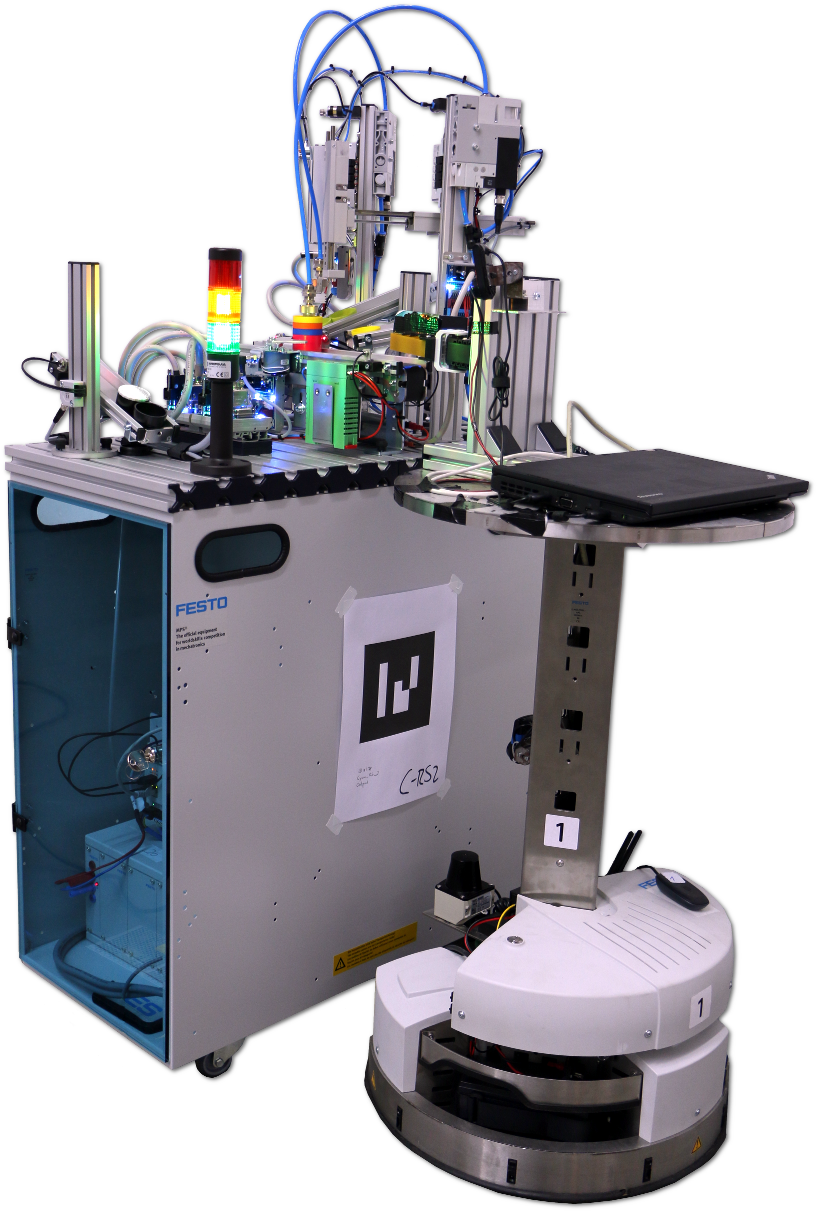
\includegraphics[width=0.3\textwidth]{img/rcll}
  \vspace{-4ex}
  \caption{Robot and MPS used in the RCLL~\cite{chapter-cps}}
  \label{fig:rcll}
\end{wrapfigure}
\reffig{fig:rcll} shows an RCLL robot filling
a machine which mounts colored rings on work pieces. The robots are
based on the Festo Robotino 3 platform which uses a holonomic drive,
and can be extended and programmed by the teams. The robot shown in
\reffig{fig:rcll} was built by the Carologistics team and uses a
laser range finder for localization, a custom made gripper for
handling work pieces, and several cameras for detection of markers and
light-signals mounted on the machines~\cite{Carologistics2015,chapter-cps}. The
game is controlled by a software component called \emph{referee box
  (refbox)} which randomizes the machine placement in the factory and
the production orders, communicates with the competing robots,
controls the machines, and awards points.

The game consists of two phases~\cite{LLSF-Rules-2015}. In the first
phase, the \emph{exploration phase}, the robots have to roam the
factory to find randomly placed machines which are used later.
%% By detecting the light signal shown by the machines, the robots can
%% determine the machine-type. For correct reports of discovered machines
%% to the refbox the team is awarded points, for incorrect ones points
%% are subtracted.
%%
%% \begin{figure}[t]
%%   \centering
%%   \begin{minipage}{.8\linewidth}
%%   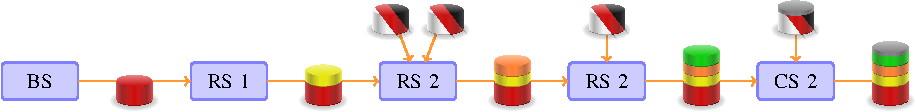
\includegraphics[width=\linewidth]{img/chain_c3}%
%%   \end{minipage}
%%   \quad%
%%   \begin{minipage}{.15\linewidth}
%%   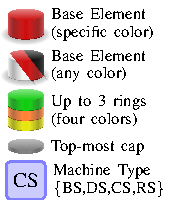
\includegraphics[width=\linewidth]{img/legend}%
%%   \end{minipage}
%%   \caption{Production chain of a high complexity
%%     product in the RCLL.}
%%   \vspace{-2mm}
%%   \label{fig:prod-chain}
%% \end{figure}
%
In the second phase, the \emph{production phase}, the refbox announces
orders, which products have to be produced by the robots. The products
are build from colored cups with optionally mounted rings and a
colored cap.
%% \reffig{fig:prod-chain} shows the production chain to
%% build a high complexity product.
There are four different machine
types. The \emph{base-station (BS)} provides new bases, the colored
cups, as raw resource. The \emph{ring stations (RS)} mounts colored
rings on a work piece
%after preparing it with a varying amount ofbases.
The \emph{cap-station (CS)} mounts %black or grey
caps to finish a product
%after loading it with a cap form a shelf first.
The \emph{delivery-station (DS)} is used to deliver products.

A major challenge of the RCLL lies in the fully autonomous task
planning and coordination of the multi-robot system in the dynamic
environment with spatial information and time constraints.
%% to build as many ordered products as possible and deliver
%% them in time given time window, and in the baseline robotic challenges
%% such as collision avoidance, perception and behavior execution. The
%% dynamism of the environment is caused by the ranomized factory layout,
%% randomized out-of-order times of machines, the highly customizable
%% amount of products that preclude producing in advance, unknown
%% obstacles, such as the other teams robots and hard to completely avoid
%% handling mistakes by the robots.
To cope with these challenges, a
multi-robot decision making is necessary and therefore a mechanism to
share knowledge about the world model between the robots. This can be
done by the robot memory which also allows combining a global planner
for finding plans and a reasoner for plan execution.

\subsubsection{RoboCup@Home League}
\begin{wrapfigure}{r}{0.3\textwidth}
  \centering
  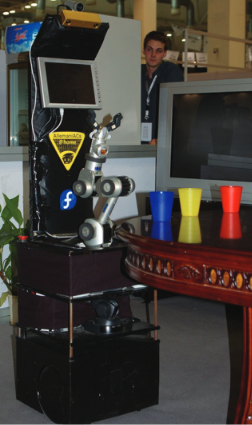
\includegraphics[height=150px]{img/ceasar}%
  \caption{RoboCup@Home robot tidying up~\cite{wisspeintner2009robocup}}
  \vspace{-2mm}
  \label{fig:athome}
\end{wrapfigure}

The RoboCup@Home league is a competition about domestic service
robots~\cite{wisspeintner2009robocup}. Robots have to assist
humans in a wide variety of everyday tasks. These tasks include
serving drinks, cleaning, setting tables, guiding or following people,
helping in emergency situations, shopping, and cooking.
\reffig{fig:athome} shows an @Home robot in the
competition.
%
The goal of the RoboCup@Home league is to foster and benchmark
research in the area of domestic service robots, to build a research
community and to envision autonomous multi-purpose robots helping
humans and especially elder people in the personal life.

The competition consists of multiple sub-tasks
such as finding and manipulating objects, navigation tasks,
remembering persons, wait on tables, acting as
nurse, and an open challenge~\cite{athome-rules}.
To solve these challenges, robots need to
have a wide variety of abilities, including navigation, object
detection and manipulation, speech recognition, and especially human
robot interaction, which requires, for example, applying everyday
knowledge to incomplete task descriptions given by humans.

Important challenges in the @Home league are acting robustly in a
dynamic and only partial observable domestic environment and hybrid
reasoning with qualitative and quantitative information.
The robot memory can help here because it allows to collect a lot
of knowledge about the concrete domestic environment and, for example,
log object observations to learn their spatio-temporal distribution.
%% Furthermore, detecting and manipulating objects in a personal
%% environment can be difficult because the space the robot acts in, for
%% example the frige, can be very clouded.

\subsection{Fawkes Robot Software Framework}
\label{sec:fawkes}
The basis for the proposed thesis is the robot software framework
\emph{Fawkes}\footnote{\url{http://www.fawkesrobotics.org}}
available as Open Source~\cite{FawkesDesign,Fawkes-RCLL-2014}.
%and developed at the Knowledge-based Systems
%Group\footnote{\url{http://www.kbsg.rwth-aachen.de}} (KBSG) at RWTH
%Aachen University
It is designed to work with
various robots in different domains and follows a component-based
software design which separates functional entities into individual
software modules~\cite{component}. This enables reusing
software solutions for robotic problems such as localization,
perception, reasoning, and behavior execution. The compiled
components can be loaded as \emph{plugins} at run-time.
%
Plugin activity is organized in threads
%to make use of multi-core architectures. The threads
which can be run continuously ore hooked into
the main-loop of Fawkes to order the execution into a
\emph{sense-think-act} cycle.
%This guarantees that higher-level components can use the latest data.
Fawkes softly guarantees loop times by
monitoring and eventually pausing and resuming threads running for too
long.
% Ros blabla from BA?
Features in Fawkes are provided as \textit{aspects}. These are
based on aspect-oriented programming~\cite{aspect_oriented} and give
access to a particular feature. Threads that need to use a feature can
inherit from the corresponding aspect. For example, there are aspects
for accessing logging, timing, and specific external libraries~\cite{tnthesis}.

The communication between plugins is realized with a \emph{hybrid blackboard}
paradigm. The blackboard lists structured entries called
\emph{interfaces} which contain qualitative and quantitative information.
Interfaces can be
provided by one plugin at a time, the writer, and read by other
plugins, the readers. This allows a very flexible communication
because the interface is independent from the concrete writer and readers.
For example, sensor and actor plugins can be exchanged by simulation
plugins~\cite{LLSF-Sim}.
%% because the information provision in the interface is decoupled from
%% the concrete components which use the information and plugins writing
%% to the interfaces can be exchanged, e.g. by simulation plugins writing
%% to the same interface. Furthermore, the blackboard architecture
%% simplifies debugging because the current communication between two
%% plugins, determined by the state of the interface, can be viewed and
%% logged at run-time.
To send commands to an interface writer, e.g. a
motor command to the motor controller, readers can send messages to
the interface.

As a communication infrastructure between different components, the
blackboard is a limited possibility to realize a robot memory.
%shared between multiple planners and reasoners in the current version of
%Fawkes.
Indeed the blackboard works well for providing information and
sending commands, though there are limitations for this
application. The size and structure of blackboard interfaces is fixed, and
thus does not allow to dynamically represent more information.
%% , such as positions
%% of detected objects, than initially defined.
Furthermore the blackboard does not support long-time memory,
expressive querying, and event-triggers.

\subsection{Planners and Reasoners}
\label{sec:planners}
This subsection gives an overview of planners and reasoners which are
going to benefit from the robot memory. For the variety of these, we
give four examples which should use the robot memory to achieve new or
improved functionality and to evaluate this thesis. The example
planner and reasoner systems are \emph{CLIPS}, a rule-based production
system, the \emph{Planning Domain Definition Language (PDDL)}, which
incorporates a family of planning formalisms into a standard
programming language, \emph{Golog}, a high-level programming language
based on the Situation Calculus, and \emph{Motion Planners} finding
collision free actuation plans.
%% These examples are representatives for often
%% used types of planners and reasoners. However, the robot memory should
%% not be limited to these examples and provide a general C++ interface.

\subsubsection{CLIPS rules engine} The reasoner currently used by
Carologistics in the RCLL
to implement the high-level game agent is the rule-based production
system CLIPS~\cite{CLIPS-RM}. It uses forward chaining based on the Rete
algorithm~\cite{Rete} and basically consists of a fact-base, which is a
working memory with small pieces of information, a knowledge base
with rules and procedures, and an inference engine
working with the knowledge base on the fact-base. The pieces of
information in the fact-base are called facts and consist of a name
and a key-value structure defined in a template for \emph{unordered
  facts}
(e.g. \textit{(position~(name~robot1)~(translation~2.5~1.0~0.0)}) or
an ordered list of values for \emph{ordered facts}.
\begin{figure}
\begin{lstlisting}[showlines,style=ReallySmallCLIPS, caption={CLIPS
    rule to change a robots state when the object it searched for is visible.},
  label=lst:clips-rule,
  emph={skill, args, state, target, res},
  emphstyle=\bfseries\color{green!80!black},
  emph={[2]\?skill, \$\?args, wait-for-lock, \?target, use,
  WAIT-FOR-LOCK, SKILL-EXECUTION, running},
  emphstyle={[2]\bfseries\color{blue!80!black}},
  morekeywords={retract, assert, modify, skill-call, skill-to-execute,
  wait-for-lock}]
(defrule found-machine
  ?s <- (state SEARCHING_FOR ?machine)
  (visible  (name ?machine))
  (position (name robot1) (translation $?pos))
  =>  
  (retract ?s) 
  (assert (state IDLE))
  (printout t "Found machine " ?machine " at " ?pos crlf)
)
\end{lstlisting} %$ This is just to fix Emacs highlighting due to dollar sign in code above
\end{figure}
An example rule is shown in \reflst{lst:clips-rule}. Rules are
composed of an \emph{antecedent} and a \emph{consequent}. The
antecedent is the first part of the rule and describes the condition that
has to be satisfied before the the rule is considered for activation.
It consists of a
list of patterns that have to be matched by facts in the fact-base. For the
antecedent in \reflst{lst:clips-rule} there have to be fitting
\texttt{state}, \texttt{visible}, and \texttt{position} facts with
matching constants and variables started with questionmarks.
The consequent is written behind the antecedent and
defines the procedure to execute when the rule is
activated. It usually modifies the fact-base by retracting and
asserting facts, for example to exchange the \texttt{state} fact.
The inference engine checks which rule antecedents are satisfied and
puts only them on the \emph{agenda}.  Which rule of the agenda is
executed, is determined by a conflict resolution strategy such as
highest priority or earliest on the agenda.  The consequent of the
chosen rule is executed and the inference engine checks
again. \emph{Functions} encode procedural knowledge, can have side
effects, and also be implemented in C++.

The Carologistics RCLL agent implemented in CLIPS represents its
knowledge about the world, the \emph{world model}, in its
fact-base. It chooses actions to taken by using a
technique called \emph{Incremental Reasoning}~\cite{CLIPS-Agent}:
Whenever the robot is idle, it searches for the
next best task and executes it.
%% For each task there is a rule with its
%% preconditions in the antecedent and the actions to take in the
%% consequent. There are also rules for modifying the world model
%% (e.g. after finishing actions or getting new sensor data), task
%% execution, coordination with other robots and more.
The coordination
of the robot team includes synchronizing their world model
%% , so each
%% robot knows what other robots noticed and changed in the environment,
and resource allocation.
%% to ensure no two robots try to use the same
%% machine at a time or try to achieve the same goal by choosing a
%% redundant task.
This coordination is currently implemented in CLIPS
rules using Google Protocol Buffers (Protobuf)
messages. Alternatively, this could also be done by using a
distributed robot memory which contains the world model in a
distributed database. This would be advantageous
because the database already provides efficient synchronization and
the implementation in CLIPS increases the agent's complexity.
%% and is not convenient because the language focuses on reasoning
%% instead of messaging and data synchronization.


\subsubsection{Planning Domain Definition Language (PDDL)} PDDL is a
standardized language for planning problems~\cite{PDDL}. It allows
modeling the nature and behavior of a domain as well as the
\emph{actions} possible to perform in a \emph{domain
  description}. With an additional \emph{problem description} which
defines the problem to solve it can be given to a PDDL planner which
typically searches for a totally or partially ordered sequence of actions, the
\emph{plan}, to solve the problem.
%% \todo{action example}
%% \reflst{lsf:pddl-action} shows an example action contained in a domain
%% description.
Actions consist of preconditions and effects.  There are
various versions and extensions of PDDL which introduce new concepts
and features. For example, PDDL~2.1~\cite{PDDL2.1} adds numeric values and
continuous actions. This allows finding plans in continuous
environments where, for example, distances and travel times
matter. PDDL has the advantage of being able to find complete and
optimal or efficient plans depending on the model. However, this comes with the
drawbacks of high computational effort for larger domains and the
problem of adopting to events during plan execution. For example when
the domain is not fully observable, the robot could sense changes in
the environment or fail executing an action. This would require
notifying the planner, incorporating the changes in PDDL and
re-planning. To solve this problem, the robot memory should allow combining PDDL with an
execution in CLIPS. Then PDDL generates an efficient and complete plan
with coarse actions and CLIPS executes the plan action for action,
while monitoring the execution and updating the world model according
to perceived changes. This world model is written into the robot
memory so that PDDL can access the world model with all changes applied.
This way the strengths of both PDDL and CLIPS are combined.


\subsubsection{Golog} Golog is a high-level programming language based on the
\emph{Situation Calculus}, a first order logic formalism for knowledge
representation and reasoning in dynamic domains~\cite{Golog}. It
allows representing world states as terms called
\emph{situations}. These are used in functions yielding new situations
(e.g. for the situation resulting from performing an action in a
situation). Relations using situations are called \emph{fluents} and
describe some property in a situation. \emph{Actions} are also
represented by terms and are modeled with preconditions and
effects. If an action is possible in a situation is defined by a
sentence, the \emph{precondition axiom}. The \emph{successor state
  axiom} is a sentence describing fluents in the situation resulting
from performing the action in a situation satisfying the precondition
axiom.

Golog as a high-level programming language features imperative
programming constructs such as procedures, conditions, and loops as
well as nondeterministic branching. There are multiple dialects of
Golog which add features needed for robotic
applications. ConGolog~\cite{ConGolog} adds concurrency and
interrupts, IndiGolog~\cite{IndiGolog} adds on-line execution of
programs and sensing actions, which determine the value of a fluent
during execution, and ReadyLog~\cite{ferrein08ras} extends IndiGolog
to support robot decision making in dynamic real-time domains. With these
dialects, Golog has been found useful for robot applications in
multiple domains such as domestic service robots. By providing an
interface to the robot memory, the strength of Golog, the highly
expressive behavior specification, can be combined with other
approaches to compensate the weaknesses, e.g. inefficient
planning~\cite{Golog-Planning}. There already are approaches to
combine Golog an PDDL into a continuous planning framework that uses
PDDL for planning and Golog for execution and expanding placeholder
actions into sub-plans based on current information unavailable during
initial planning~\cite{ContPlanGolog}. It is implemented with a
translation between PDDL and
Golog~\cite{Golog-PDDL-Trans}. Furthermore, the robot memory could be
useful as additional persistent and distributed knowledge storage
(e.g. for saving the context during an interrupt~\cite{Gesche-Thesis}).

\subsubsection{Motion Planners}
Another kind of widely used planners in robotics are geometric motion
planners. They usually plan the motion of a robotic arm or the path
of a driving robot to reach a certain goal position where an object
should be grabbed or the robot wants to go to. Thus they use geometric
knowledge in contrast to logical reasoners and planners focusing on
symbolic knowledge.
A motion planner needs to find a trajectory from the initial position to
the goal position, taking joints of the arm into account and avoiding
collisions with objects in the environment. A widely used motion
planner framework is MoveIt! which is available for ROS~\cite{MoveIt}.
Another motion planner framework already integrated into
Fawkes is OpenRave~\cite{OpenRave}. These planners could benefit from
using a robot memory by accessing and sharing information about
objects and obstacles in the environment and by informing other
planners and task execution components about the outcome of a motion
plan (e.g. about the cause that prohibited the motion). This
especially requires the robot memory to represent hybrid knowledge in
the form of continuous positions and time related events.

\subsection{MongoDB}
\label{sec:mongodb}

%% Since storing, keeping and retrieving knowledge of the robot memory
%% are central tasks of this thesis, the choise of a database
%% implementation is important.
MongoDB is a \emph{document-oriented}
database which fits particularly well for the application in this thesis. It
provides many useful features such as flexible data structures, aggregation,
and distribution over multiple machines, which would take a large effort to
implement manually. It has proven as powerful and scalable data
storage~\cite{mongodb,RoboDB} and is widely used. In contrast to
relational databases, document-oriented ones store entities called
\emph{documents} consisting of key-value pairs.
\begin{figure}
  \begin{minipage}{0.6\linewidth}
\begin{lstlisting}[style=SmallJSON,
  caption={MongoDB document representing\protect\\ the position of a robot},
  label=lst:mongo-document,
  framexleftmargin=2pt, xleftmargin=2pt,
 morekeywords={}, numbers=none]
 {
   _id: ObjectId("573e7cfbb2af949d9"),
   type: "position",
   name: "robot1",
   translation: {x:2.5, y:1.0, z:0.0},
   rotation: {x:0.0, y:0.0, z:0.0, w:1.0},
   timestamp : ISODate("2016-05-19T15:26:34.466Z")
 }
\end{lstlisting}
  \end{minipage}
  \begin{minipage}{0.4\linewidth}
\begin{lstlisting}[style=SmallJSON,
  caption={MongoDB query yielding the document in \reflst{lst:mongo-document}},
  label=lst:mongo-query,
  framexleftmargin=2pt, xleftmargin=10pt,
 morekeywords={}, numbers=none]
db.positions.find(
  {
    type: "position",
    name: "robot1",
    timestamp : {"$gt": ISODate(
      "2016-05-19T15:26:34.000Z")}
  })
\end{lstlisting}
  \end{minipage}
\end{figure}
\reflst{lst:mongo-document} shows such a document.
%used for storing the position of a robot.
The different
values can be accessed by their key and can have different types, such
as strings, numbers, complex objects (e.g. dates) and nested
sub-documents (e.g. translation containing 3D coordinates). In
contrast to relational databases, there is no predefined schema that
enforces the structure of documents. However, documents with similar
structure are usually grouped into \emph{collections}. Therefore the
documents inserted in a collection implicitly define the structure
during run-time. This allows a flexible use of the database because
applications are not limited to a fixed schema and can, for example,
add key-value pairs during run-time when additional information needs
to be stored.
%% Furthermore, this simlyfies development in which the
%% document structure tends to change often. Even if there are documents
%% with different structure, the application can choose to retrieve only
%% certain documents by giving a specialized query.
Queries in MongoDB are similar to documents because the arguments of
query functions also use document structure. An example query is
shown in \reflst{lst:mongo-query}. It searches for all documents in
the collection \texttt{positions}
%of the current database
that have matching values for \texttt{type} and \texttt{position}, and
are up to date, thus with a timestamp greater than the given
one. Multiple key-value pairs in a query are conjunctive.  Values can
be checked and compared as in the example with a variety of operators
such as \textit{not}, \textit{or}, \textit{equals}, \textit{greater
  than}, etc. These queries can be evaluated very quickly, especially
when \emph{indexing} is used, a database feature that manages indexes
for a combination of document keys. For more complex queries it is
possible to add arbitrary JavaScript functions with the \textit{where}
operator to check if documents match the query. Furthermore, it is
possible to aggregate results using the \emph{Map-Reduce}
paradigm~\cite{mapreduce} which maps resulting documents to
intermediate documents which are then reduced until the end-result is
found. For example this allows querying for the nearest visible object
by getting all visible objects, mapping their position to a distance
and reducing them to the nearest one by dropping more distant ones
when comparing them.  The higher expressiveness of these queries comes
with the price of slower computation. However, the computational
effort can be reduced by formulating queries smartly. Many usual
queries, e.g. \reflst{lst:mongo-query}, can be formulated without
using \textit{where} operators. Furthermore, complex queries can be
nested to filter documents first with a fast query and execute the
computationally costly query only on the remaining documents.
%
An especially useful feature of MongoDB which allows sharing knowledge
between multiple robots is \emph{replication}. Replication is a
process that distributes a database onto multiple machines.
One MongoDB instance called \emph{Master} initially
copies the database  to other instances called \emph{Slaves}.
Afterwards, all modifications to the master database, which are
stored in a separate collection called \emph{operations log (oplog)}, are forwarded to
the slave to keep them synchronized and consistent.
%% This is often used
%% in web-services to distribute read-queries and their computation on
%% multiple machines and to keep backups.
Read only queries can be
computed by Master and Slave instances, modifying queries are
forwarded to the Master to guarantee consistency.
MongoDB can also group multiple
instances into a \emph{Replica Sets} which automatically manages
the master election when necessary. Using replication,
multiple robots can robustly share a common and consistent world
model. Robot specific knowledge can be kept in a separate and not
replicated collection to avoid unneeded communication.
%% There also exist
%% extensions of MongoDB which implement a \emph{Multi-Master
%%   Replication}. This would enable writing to each instance immediately
%% and synchronizing the changes later. \todo{source} This allows faster
%% writing especially if the Master is not available for some time but
%% requires to resolve write conflicts and handle them in the
%% application. Thus Master-Slave Replication is more convinient for the
%% applicaiton.
%% There are also extensions of MongoDB providing so called \emph{Trigers} which
%% can notify an application if something in the database changes as
%% previouly defined. \todo{source} These Triggers use the oplog of
%% MongoDB to find changes and are useful for planners. For example if a
%% global planner determined a plan that is being executed and wants to
%% be notified, if a condition changes that makes the plan invalid, to
%% replan.

MongoDB is especially well suited for this thesis because of its
performance and scalability compared to other document-oriented
databases with similar features. A possible alternative to MongoDB is
the document-oriented database CouchDB~\cite{CouchDB}. CouchDB
focuses more on distributed Systems providing a system called
Multi-Master Replication which allows writing to all replication instances.
Conflicts can be solved similar to a version
control system, thus multiple conflicting versions can be kept in
parallel for later revision. However, MongoDB has shown to scale much
better than CouchDB and other document-oriented databases~\cite{db-comparison}.

%% \begin{itemize}
%% \item BSON JSON format for documents
%% \item JavaScript example
%% \item Capped collections?
%% \item dreieck comparison ?
%% \item GridFS file storage?
%% \end{itemize}

\section{Related Work}
\label{sec:related}
This section gives an overview of the related work of the proposed
thesis starting with the knowledge processing systems KnowRob and
OpenRobots Ontology, which provide similar functionality. Afterwards
we present the Generic Robot Database based on MongoDB and Fawkes and
Open-EASE, a combination of KnowRob and the Generic Robot Database.

\subsection{KnowRob}
\label{sec:knowrob}
KnowRob is an open source knowledge processing system for
cognition-enabled robots~\cite{KnowRob,KnowRob-Representation}. It is
designed to store knowledge about the environment and set it into
relation to common sense knowledge to understand vaguely described
tasks such as "set the table". For representation and inference of knowledge,
KnowRob uses Description Logic and approaches of the semantic web.
%% , an effort to make websites machine understandable,
Each small piece of
information is represented as a \emph{Resource Description Framework
  (RDF) triple} (e.g. $rdf(robot, holding, cup)$) which are composed
of a subject, predicate, and object. A set of these RDF triples in a
network can compose commonsense knowledge based on the
\emph{Web Ontology Language (OWL)}. It uses
\emph{ontologies} which can roughly be described as directed graphs
setting objects or classes of objects into relation. The graph can be
represented with multiple RDF triples, where the subject and object
are nodes and the predicate is a directed edge from the subject to the
object. In these ontologies it is possible to represent common sense
knowledge such as "milk is-a perishable", "refrigerator
storage-place-for perishable", and "refrigerator is-a
box-container". Thus a robot asked to bring milk could infer that the
milk is stored in the refrigerator which needs to be opened first
since it is a box-like container. To be able to interface with
perception, KnowRob uses a concept called
\emph{virtual knowledge base}. It allows computing needed information
on demand instead of storing everything providently. Thus special
queries can be forwarded to other components which compute the answer
efficiently.
%% Especially for perception based on sensor data or
%% transformation of spatial relations, this is advantageous compared
%% to continuously computing the results for all possible queries and
%% storing them.
The concept inspired the usage of computables in this thesis.  The
implementation and interface of KnowRob is based on the logic
programming language Prolog which makes representing RDF triples and
inference with ontologies intuitive.
%% KnowRob implements it with Prolog predicates
%% called \emph{Computables} which call C++ functions of other
%% components. This indeed slows down the computation of a query but is
%% more efficient than continuously computing and storing the results or
%% implementing and computing the other components algorithms in Prolog.
To understand the robots environment large and detailed ontologies are
necessary. KnowRob features acquiring and connecting these from
various sources such as online common sense databases, the cloud-based
robot infrastructure RoboEarth and websites for
deriving object information from internet shops and action recipes
from how-to websites giving step by step instructions.
However, it has been found that this acquired
knowledge needs a lot of manual extension and verification before it
can be used~\cite{KnowRob-Web}. Encyclopedic knowledge often lacks
action information needed by the robot. %% (e.g. how to grab tools) and
%% action recipes require human text understanding
%% \todo{executive integration}
%
Furthermore large ontologies limit the performance of KnowRob because
of the Prolog implementation and general complexity. In contrast to
the robot memory intendet in this thesis, KnowRob focuses on common
sense reasoning instead of an efficient and flexible on-line
back-end. It does not support sharing knowledge between multiple
robots and has a too strong focus on data only usable for reasoning
components. Although it can also represent spatio-temporal knowledge,
we have performance and scalability concerns with Prolog handling
larger data-sets (e.g. for storing locations of found object over long
time to learn the distribution where they can be found).

\subsection{OpenRobots Ontology (ORO)}
\label{sec:oro}
The OpenRobots Ontology (ORO) is an open source knowledge processing
framework for robotics~\cite{Oro}. It is designed to enable human-robot
interaction by featureing commonsense ontologies similar to KnowRob and
modeling the human point of view. It also uses RDF triples and OWL ontologies.
The triple storage is implemented in Jena, a Java toolkit for RDF, and the
inference with Pellet, a Java OWL reasoner. Besides knowledge storing,
querying and reasoning, ORO features a modular architecture between
the back-end storage and front end socket server for querying. These
modules add features such as events that notify external components
about changes.
%%  (e.g. if instances of certain classes are added or modified).
%% \todo{executive integration}
Another module adds representations of alternative perspectives that
should allow understanding the point of view of other agents.
For example when a human asks a robot to bring the
cup, there are two cups on a table and the robot should infer which
cup is meant by knowing that the other cup is occluded from the humans
point of view. Furthermore ORO features categorization to find
differences between objects (e.g. to ask if the blue cup or the red
cup was meant in a vague task description) and Memory profiles for
distinguishing long-term knowledge and short-term knowledge which is
removed when the lifetime of a fact expires. Although these are useful
features and we want to realize the concepts of events and memory
profiles in this thesis, we do not use ORO as a basis. Due to its
focus on human-robot interaction and commonsense reasoning, it is not
suitable for representing large amounts of data for non-reasoning
components because all data would have to be stored in RDF triples and
processed by the OWL reasoner. Furthermore, it does neither support
synchronizing a part of the knowledge with other robots nor computables.

\subsection{Generic Robot Database with MongoDB}
\label{sec:mongo-logging}
There already is a generic robot database developed with MongoDB as
data storage~\cite{RoboDB}. It is used to log data of a
robot middleware (Fawkes and ROS) and allows, for example, fault analysis and performance
evaluation. To achieve this, it taps into the messaging infrastructure
in ROS and the blackboard interfaces in Fawkes to store the data one
to one utilizing the flexibility of the schema free MongoDB. The
logged data can later be queried by the robot or a developer. This
allows better evaluation and fault analysis because the data would
otherwise be disposed and logging of the whole
Data-Information-Knowledge-Wisdom (DIKW) hierarchy~\cite{DIKW} enables
retracing processes such as from point clouds (data) to cluster
positions (information) to object positions (knowledge) combined from
multiple clues to learning results (wisdom). This work already
implemented a basic connection to MongoDB in Fawkes for storing
documents and executing queries, which can be used in this thesis. It
also showed that MongoDB is a good choice because it can handle
querying a large database and writing a lot of data efficiently while
being flexible how and which kind of data is being represented.
However this work lacks some important concepts needed for a robot
memory as intended in this thesis. It is intended as logging facility
and not as working memory holding a world model for multiple planners
and reasoners. Therefore updating and querying mechanisms for planners
and reasoners are missing as well as triggers, a virtual knowledge
base, multi-robot synchronization and a suitable front-end.

\subsection{Open-EASE}
\label{sec:openease}
Open-EASE is a knowledge processing service for robots and AI
researchers~\cite{OpenEASE}. It is based on and combines
KnowRob~\cite{KnowRob} and the Generic Robot Database with MongoDB in
ROS~\cite{RoboDB}. It is designed as a web service accessible by
robots via a socket connection and by humans via a web browser. It
uses KnowRob for commonsense reasoning and storing the world model of
a robot. The Generic Robot Database is used to log data about robots
or humans performing manipulation tasks. This data can then be
accessed by using the virtual knowledge base concept to
learn from human demonstration and analyze and learn from faults. The
focus of Open-EASE also is on providing the recorded data and access
to KnowRob to humans using the web interface. This allows using
Open-EASE as eLearning tool for students, who can explore and
experiment with the data and system on the robot. Furthermore it
fosters reproducing experiment results (e.g. for reviews) and
visualizing them. Although the system is accessible from multiple
users and robots which can query the same Open-EASE instance, it is
focused on single robot data and non collaborative processes because
each user operates in his private container with individual knowledge
base. This makes sense in the context of student exercises. If the
system is also usable or being extended for cooperating robots or
planners exchanging knowledge over the web service is not mentioned in
current publications or on the project
website\footnote{\url{http://www.open-ease.org/}}.


\section{Approach}
\label{sec:approach}
This section presents the approach of the proposed thesis. It starts
with the goals we want to achieve with the robot memory and a
theoretical foundation of the robot memory and how knowledge is
transfered into a planner or reasoner. It follows an overview of the
architecture which describes in which components the robot memory is
organized and how they interact with each other. Afterwards, we
describe how the implementation is planned, especially for the robot
memory and interfaces for planners, reasoners and other components.

\subsection{Goals}
\label{sec:goals}

This subsection presents the goals of this thesis:

\smallskip
\textbf{Flexible Storage and Retrieval:} The robot memory has to
provide a service for storing, updating, removing, and querying knowledge
so that different components can use the robot memory to provide knowledge,
use it as a source, or collaborate using the same memory. It should be
flexible enough to store any kind of data, information, knowledge, and
wisdom of the DIKW hierarchy in any structure. For example the robot
memory should be able to store a world model, perception results and
even large datasets such as remembered sights of objects.

\smallskip
\textbf{Consistent Knowledge Sharing between Planners and Reasoners:}
The robot memory has to allow multiple components to collaborate by
consistently sharing a common database. This should especially be used
to share a common world model between different kinds of planners and
reasoners.  This allows combining them with their specialided
strengths (e.g. generating plans in PDDL and executing them in CLIPS).
It avoids inconsistencies because the knowledge used by the planner or
reasoner is generated by the robot memory and thus only one state
estimation is necessary. For example world model changes detected and
stored in the robot memory by CLIPS are made available to PDDL.

\smallskip
\textbf{Special Views for Different Components:} Depending on the
application of different components using the robot memory, different
views on the stored data is necessary. For example a planning
components needs another part of the stored data, than a component
learning distributions of object sights. Thus component-specific
filters are necessary. Furthermore, different components need the
stored data in different formats (e.g. depending on the used
programming language). Keys or identifiers might be named differently
and have to be translated.

\smallskip
\textbf{Knowledge Computation on Demand:} With computables, the robot
memory has to provide knowledge on demand. This is knowledge that is
not stored in the robot memory directly, but computed when
needed. This allows accessing knowledge through the robot memory that
is otherwise impracticable to compute and store continuously and for
all possible queries. For example when a component queries the
distance of two objects, it is better to compute the result on demand
than to store all distances between each two objects in the memory and
to keep them updated. When components using the robot memory can also
provide computables to the robot memory, this adds a lot of
versatility and expandability. To lower the computational effort of
processing the same querry frequently it would be possible to add
time-bounded caching for computed knowledge.
%% For example it would be possible to add
%% a commonsense reasoner similar to KnowRob or ORO providing computables
%% to the robot memory. Queries for this commonsense knowledge would then
%% be forwarded to the commonsense reasoner and be solved by relating
%% knowledge in the memory to an ontology.

\smallskip
\textbf{Shared Knowledge for Multi-Robot Systems:} The robot memory
should be able to distribute parts of the knowledge over multiple
robots, which can then share a common world model necessary for
collaboration. The concept is similar to multiple planners sharing a
world model on the same machine with the difference that the
components on a multi-robot system work simultaneously and the
additional difficulty of message loss and keeping consistency. Such a
distributed robot-memory is necessary in many multi-robot domains,
especially in the RoboCup Logistics League (RCLL).
%%  where the whole robot team needs to know the world model
%% (e.g. where other robots placed intermediate products) and what other
%% robots intend to achieve at the moment.
%% If the distribution of the
%% knowledge would not be implemented in the robot memory it would have
%% to be implemented separately. 
Distributing the robot memory adds
additional requirements and challenges, especially robustness (e.g. in
the case of robots dropping out), consistency of the memory, and
accessibility so each robot can use the robot memory without large
latices.

\smallskip
\textbf{Spatio-Temporal Grounding:} It is often desirable to ground
stored knowledge based on location and time because this is the
prerequisite for many applications such as spatio-temporal clustering
and learning distributions (e.g. at which day-times objects can be
found at which positions~\cite{deebul}). Thus the robot
memory has to be able to store knowledge tagged with spatio-temporal
information and consider this information while querying.

\smallskip
\textbf{Event Triggers:} The robot memory should be able to notify
components about relevant changes in the memory.  These notifications
are called \emph{event-triggers} and should automatically be sent
after a component registers an event it wants to be notified
about. These events include appearances of new instances of a specific
knowledge type, modifications and deletions of it, as well as
sentences becoming true or queries returning documents. The balance of
expressiveness versus performance still needs to be found. An examle
use case, in which event triggers are useful, is updating planner
predicates.

\smallskip
\textbf{Modular Extensions:} The robot memory should be expandable
with modules to implement additional functionality. An example module
could introduce knowledge decay for removing knowledge with exceeded
lifetimes. This would allow differentiating short-term knowledge and
long-term knowledge. Other modules could, for example, reset a part of
the robot memory to an initial state or add confidence values to
stored knowledge.

\smallskip
\textbf{Persistent Storage:} To profit from long-time knowledge and to
operate robots over long time as necessary in intended domains
such as the domestic service, the knowledge needs to be stored
persistently. This way, it is not lost when restarting a robot or
repeating an experiment depending on knowledge stored in the robot
memory.

\smallskip
\textbf{Human Interface and Visualization:} An important factor in the
development of a robotic systems is the accessibility of underlying
components for easier debugging and modeling. Therefore the robot
memory needs to provide an interface for developers to introspect and
modify the state represented in the robot memory. A visualization
would also be desirable to analyze spatio-temporal data efficiently.

\subsection{Theoratical Foundation}
\label{sec:formalism}
In this subsection, we lay the theoretical foundation for the robot
memory and the integration into planner and reasoner languages. For
this proposal we focus on the integration into PDDL. 
The formal definition of the robot memory describes how knowledge is
represented and depends on the definition of computables. Because the
robot memory is document oriented, we first define documents and their
key-value pairs. This definition is derived from the specification of
the Binary JavaScript Object Notation
(BSON)\footnote{\url{http://bsonspec.org/spec.html}} used in MongoDB.
Because documents can be nested, we define them by induction. Unnested
documents are defined as follows:
\begin{enumerate}
\item \textbf{Keys} are strings $\mathcal{K} := \Sigma^*$, where
  $\Sigma$ contains all valid symbols.
\item  \textbf{Atomic values} $\mathcal{V}_0$ are constants containing
  integers, floating point numbers, and strings.
\item \textbf{Unnested key-value pairs:} $\mathcal{P}_0:=\mathcal{K}\times\mathcal{V}_0$
\item \textbf{Unnested documents} are sets of key-value pairs with
  unique keys and thus included in the power set of $\mathcal{P}_0$:\\
  $\mathcal{D}_0:=\{
  d\in\mathbb{P}(\mathcal{P}_0)|
  \forall (k,v),(k',v')\in d , k\neq k' \vee (k,v)=(k',v')
  \}$
\end{enumerate}
Values and documents with a nesting depth up to $n$ with $n>=1$ can be
defined as follows:
\begin{enumerate}
\item  \textbf{Values:} $\mathcal{V}_n := \mathcal{V}_{n-1} \cup \mathcal{D}_{n-1}$
\item \textbf{Key-value pairs:} $\mathcal{P}_n:=\mathcal{K}\times\mathcal{V}_n$
\item \textbf{Documents:}
  $\mathcal{D}_n:=\{
  d\in\mathbb{P}(\mathcal{P}_n)|
  \forall (k,v),(k',v')\in d , k\neq k' \vee (k,v)=(k',v')
  \}$
\end{enumerate}
This yields the set of all \textbf{finitely nested documents}
$\mathcal{D}=\cup_{n\in\mathbb{N}}\mathcal{D}_n$. Infinite nesting and
documents containing themself are not considered because they are not
supported by the underlaying database implementation.
\\
A \textbf{database} is a set of documents $\mathcal{DB} \subset \mathcal{D}$.
%% with unique object
%% identifiers, which are a special key-value pair:
%% \begin{align*}
%% \mathcal{DB} \subset & \{d\in\mathcal{D} | ("\_id",v)\in d\},\\
%% & \text{where } \forall d,d' \in \mathcal{DB} \text{ with } ("\_id",v)\in
%% d \text{ and } ("\_id",v')\in d' , d=d' \vee v\neq v'
%% \end{align*}
\textbf{Queries} are represented by documents $q\in\mathcal{D}$ and yield a set
of documents $r\subset\mathcal{DB}$ as result when executed in a database according a
specification (e.g. of MongoDB~\cite{mongodb}).
\\
A \textbf{computable} $f$ is a function mapping a query document to a
set of computed documents
$$f: \mathcal{D} \rightarrow \mathbb{P}(\mathcal{D})\text{.}$$
%
With these preliminaries, we can now define a \textbf{robot memory} as tuple
of a database~$\mathcal{DB}$ and a set of computables~$\mathcal{C}$:
$$\mathcal{RM}=(\mathcal{DB},\mathcal{C})$$
%
The set of documents \textbf{memorized} by the robot memory consists
of the underlying database and all computable documents:
$$mem(\mathcal{RM})=DB \cup \bigcup_{f\in\mathcal{C}}f(\mathcal{D})$$

To integrate the robot memory into PDDL, we need to define the
\textbf{mapping functions} $map_d$ between documents and predicates, and
$map_v$ between values and terms. As prequisite, the connection
between key-names in documents and predicates, functions, and their
attributes needs to be defined. Let $\mathcal{R}$ be the \textbf{set
  of predicate symbols} and $\mathcal{F}$ be the \textbf{set of function
  symbols}, then
%
$$name_{predicate}: \mathcal{R} \rightarrow \mathcal{K}
\text{ and } name_{function}: \mathcal{F} \rightarrow \mathcal{K}$$
%
map to the strings used in document keys
(e.g. $name_{predicate}(\text{at})="\text{at}"$). The functions
%
$$ name_{func-atr}: \mathcal{R} \times \mathbb{N} \rightarrow
\mathcal{K}
\text{ and } name_{pre-atr}: \mathcal{F} \times \mathbb{N} \rightarrow
\mathcal{K}$$
%
map the attributes in the predicate or function to a key
name (e.g. $name_{pre-atr}(\text{at},1)="\text{object}"$ and
$name_{pre-atr}(\text{at},2)="\text{room}"$).
\\
Now we can define the mapping of values in documents to terms as
follows. Values which are no sub-documents can be mapped directly to
the corresponding constant:
$$map_f(v)=v, v \in \mathcal{V} \setminus \mathcal{D}$$
Otherwise the value is a sub-document, whis is mapped to a function term:
\begin{align*}
  map_f(d)= &\text{ }f(map_f(v_1), ..., map_f(v_n)), \text{ iff } f \text{ is a n-array function in } \mathcal{F},\\
  &("function", name_{function}(f))\in d,
  \forall i \in \{1..n\} (name_{func-atr}(f,i), v_i)\in d\\
  map_f(d)= &\text{ } nil_f, otherwise\text{~~~~~~~~~~~~~~~}
\end{align*}
where $nil_f$ is a new constant used for unmapable documents.
Similarly documents can be mapped to predicates as follows:
\begin{align*}
  map_p(d)=&\text{ }p(map_f(v_1), ..., map_f(v_n)), \text{ iff } p \text{ is a n-array predicate in } \mathcal{R},\\
  &("predicate", name_{predicate}(p))\in d,
  \forall i \in \{1..n\} (name_{pre-atr}(p,i), v_i)\in d\\
  map_p(d)=& \text{ }nil_p, otherwise\text{~~~~~~~~~~~~~~~}
\end{align*}
For example is
\begin{align*}
map_p&(\{("predicate", "at"),("at\_object", "cup"),("at\_room",
"kitchen")\})\\
&= at(map_f("cup"), map_f("kitchen")) = at(cup, kitchen) \text{.}
\end{align*}
This theoretical foundation of the robot memory and the mapping of
queried documents into predicates is the basis for the generation of
PDDL problem descriptions. In future work, this can also be used to
formalize the integration of the robot memory into Golog, but this
exceeds the scope of the proposed thesis.

\subsection{Architecture}
\label{sec:arch}
This subsection presents the architecture of the robot memory and
explains its design considerations. It shows how the intended
functionality is organized in smaller components and how these
components interact with each other. The architecture contains
standard concepts of software engineering, most importantly a layered
architecture, functional abstraction, and data
abstraction~\cite{software-architecture}, to allow
reusability and adaptability to changing requirements and use cases.
%% functional abstraction,
%% %% (e.g. of the different processes happening during storing and
%% %% querying)
%% and data abstraction.
%% %%  (e.g. of stored knowledge which is
%% %% more specialized internally than visible from a using
%% %% application)

\reffig{fig:arch} shows the architecture of the robot
memory and is explained in the following.
\begin{figure}
  \centering
  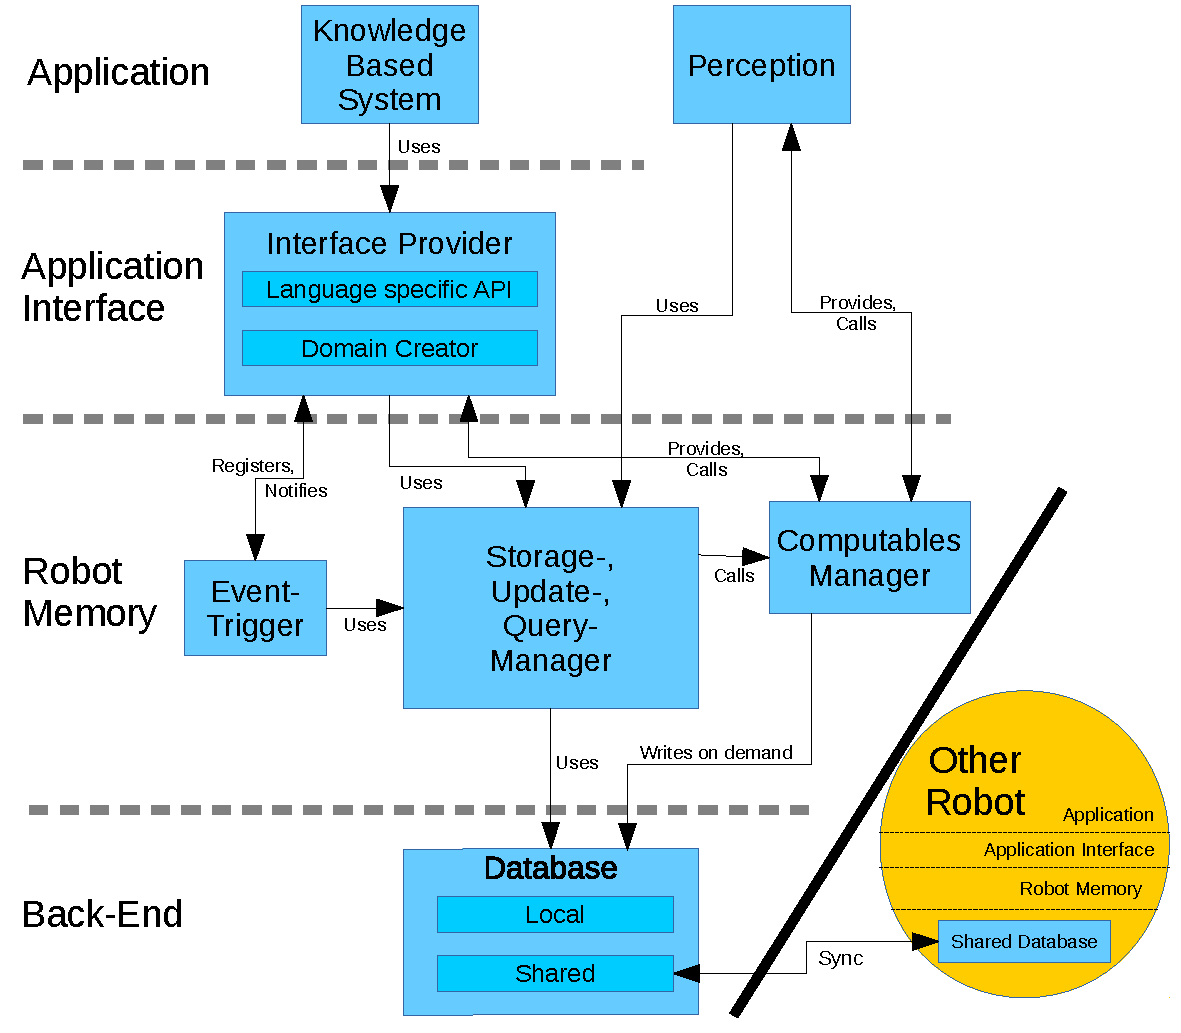
\includegraphics[width=0.9\textwidth]{architecture.pdf}
  \vspace{-5mm}
  \caption{Software architecture of the Robot Memory}
  \label{fig:arch}
  \vspace{-5mm}
\end{figure}
The architecture organizes all components into four layers: Back-End,
Robot Memory, Application Interface, and Application. The Back-End
contains a databases for storing knowledge and executing
queries. There is a private part and a shared part distributed between
multiple robots using the same architecture. This distribution can
utilize the replication features of the databese. The Robot
Memory-layer contains the central functions that distinguish the robot
memory from a pure database. It contains the Storage-, Update-, and
Query-manager which is an intermediate component that realizes most of
the robot memorys functionality by modifying and enhancing queries,
storage and update requests before applying them to the database. If a
query asks for virtual knowledge, the manager forwards it to the
computable manager, which manages which computable is provided by
which application and requests the computation on demanded. The
component responsible for event-triggers receives and manages
registrations of applications that want to be notified in the case of
an event. It uses the Query-manager to check if events happen and
notifies applications accordingly. Additional modules can be added to
extend the functionality of the Storage-, Update-, and
Query-manager.
%% These extensions can use the Command Pattern~\cite{design-patterns}
%% and to work process compositionally and dynamically.
Between the robot memory and a planner (or reasoner) components is the
Application Interface layer. For each planner language, it includes a
Interface Provider component, which makes the function of the robot
memory available to the planner and the special programming language
used. It is not necessary for components that can directly use the C++
interface of the robot memory. The responsibilities of the interface
provider also include transforming query results in the appropriate
format used by the planner and eventually renaming key-names if they
have be mapped to match the names used in the planner domain
model. Because planning and reasoning languages and concepts can be
very different, each planner and reasoner needs a separate Interface
Provider. The Interface Provider can also contain a domain creator,
which creates an initial state (e.g. a problem definition or initial
fact base) from a template and additional knowledge resulting from
queries. Finally the Application layer contains all components using
the robot memory either through the Interface provider or directly
through the robot memory interface. Application components can also
register event-triggers and provide computation functions for
computables. The sources and consumers of knowledge stored in the
robot memory are the applications using it. The ordinary data flow
starts in the application requesting storage, modification, or
querying of knowledge (over the language specific interface). The
Storage-, Update-, and Query-manager forwards the request enhanced
with management information to the database. For queries, the result
is transfered back on the reversed path of the query request. For
computables, the only difference in the dataflow is the knwledge
computation before executing the query in the database. The Storage-,
Update-, and Query-manager additionally initiates the knowledge
computation via the Computables Manager, which forwards the query to
the application providing the specific computable. The application
then computes and stores the result in the robot memory, where it is
queried afterwards.
%% Additionally the Initializer module can
%% provide the initial knowledge from a file (e.g. for the world model of
%% a new RCLL game).


\subsection{Implementation}
\label{sec:impl}
This subsection covers the considerations for the implementation. It is
separated according to the layered architecture. Both application
layers are represented by the planner and reasoner part, because all
other application components (e.g. for perception) can simply use the
C++ interface of the robot memory.

\subsubsection{Back-End}
\label{sec:back-end}
The back-end is realized with MongoDB. It acts as storage of the robot
memory, and executes queries. The representation of stored knowledge
utilizes the document structure of MongoDB with key-value pairs and
nested sub-documents. This allows a very flexible storage of
knowledge-pieces in the structure induced by the application and
expandable by robot memory information.
\begin{wrapfigure}{r}{0.47\textwidth}
\begin{lstlisting}[style=SmallJSON,
  caption={Representation of a knowledge piece in the back-end},
  label=lst:backend,
  framexleftmargin=1pt, xleftmargin=0pt,
 morekeywords={}, numbers=none]
 {
   _id: ObjectId("983e7c49h5"),
   _robot_memory_info:
   {
     persistent: true,
     decay_time: ISODate("2016-05-19T
                   23:50:00.000Z")
   },
   type: "object info",
   name: "milk_1",
   position: {x:2.5, y:1.0, z:0.0},
   storage_place: "refrigerator"
 }
\end{lstlisting}
\end{wrapfigure}
An example document stored in the back-end is shown in
\reflst{lst:backend}.  It contains knowledge about a bottle of milk as
it could be needed by a planner with additional information where it
should be stored later. Additionally the document contains meta
information needed by the robot memory (e.g. if the document should be
stored persistently or removed at restart and when it should be
dropped because it's use-time has expired). The MongoDB back-end also
manages the distribution of knowledge between multiple robots. A part
of the robot memory is only locally relevant. The other part that
should be shared has to be set up as MongoDB replica set as already
described in \refsec{sec:mongodb}. This ensures that no unnecessary
data is sent over the network. The other problems of a distributed
database such as consistency, master election and synchronization are
solved by MongoDB using replication. The back-end also contains the
operations log (oplog) of MongoDB, a separate
%% capped
collection containing a list of all changes to the database with a
timestamp. This can also be accessed by the robot memory to analyze
changes (e.g. for event-trigger).

\subsubsection{Robot Memory}
\label{sec:impl-memory}
The robot memory middle-layer implements most functions exceeding a
typical database.
%% between the
%% applications storing and querying knowledge and the MongoDB back-end
%% is an important part of the thesis because most of the functions
%% exceeding a typical database are realized here.
A central question is which query language should be used between
applications and the robot memory because this determines the
expressiveness and has a large impact on the performance. We choose to
use the query language of MongoDB as it is already used between the
robot memory and the back-end. This has many advantages compared to
using other query languages such as SQL, SPARQL,
XQuery~\cite{query-languages}, and JSONiq~\cite{jsoniq}.
%
For the application view, the query language of MongoDB is a good
choice because it is an intuitive query language, has been proven as
efficient for usual and well designed queries, and is also highly
expressive when using additional JavaScript functions or the MapReduce
paradigm~\cite{mongodb,RoboDB}. For the robot memory, it requires no
translation before application on the database and is very flexible
for extending and modifying queries because queries are structured as
documents with key-value fields and can be nested or executed in
sequence. Furthermore, MongoDB queries can easily be parsed (e.g. from
a string) by using the MongoDB C++ API. The resulting object can be
analyzed and modified for example to add key-value pairs or to check
if computables are queried.

This provides the starting point for the Storage-, Update-, and
Query-manager. When adding new documents, the
\texttt{robot\_memory\_info} sub-document can be added to store
additional meta information. When querying documents, this information
can be removed by using a filter. To detect queries for computables,
the manager can analyze the fields of the query to check if there is a
computable provided for it.  For example when a query contains the
field \texttt{type:"distance"} and there is a application that
provides computation functions for distances between two objects, the
query can be forwarded with the additional parameters, the two
objects.  When some fields are missing (e.g. only one object is given)
the application may have to compute all distances, so that the query
can afterwards be executed on the set of results (e.g. to find the
nearest one with some property). To execute the query as a usual query
with arbitrary filters, aggregation and functions, the computation
function writes the the result into a separate collection the query
can be executed on with MongoDB. We have verified this concept using a
prototype, which executes queries from interface messages either on
the MongoDB directly or in case of computables about other interfaces,
generates the knowledge from the blackboard on demand and then
executes the query.

To implement event-triggers, a registration function needs to be
provided that takes a notification function and a query to define the
event. This query can check the oplog first whether there are changed
documents with relevant key-value pairs and afterwards execute a more
complex query on the database. The registration also specifies whether
the callback function is called if the query result changes, returns
no document, or is not empty. Whether event-triggers on computables
perform well, has to be evaluated. It would be possible to allow
events only on knowledge in the database or to compute the knowledge
and check for the event in certain intervals while monitoring the
computation time.

Modules extend the functionality of the robot memory. For
implementation, they can be called periodically or with hook-points at
major steps of the robot memory such as initialization and query
execution. For example, a knowledge decay module could use cronjob to
remove documents with exceeded lifetimes in certain intervals. Further
hook-points would be at query-modification time (e.g. to add
additional meta-information) and at query-result-return time (e.g. to
filter or modify resulting documents).

\subsubsection{Planner/Reasoner}
\label{sec:impl-planner}
The implementation on the application layer includes the development
of the Interface Provider and the usage of the robot memory in the
planning language. As an example for the various planners and
reasoners, we focus here on CLIPS. The Interface Provider for CLIPS
can be realized as CLIPS-feature in Fawkes as it was already done for
providing CLIPS access to the blackboard, Profobuf-messaging and the
navgraph. The CLIPS \emph{robot-memory feature} will be implemented in C++
and provides the CLIPS environment with functions that call C++
functions of the robot-memory feature. For example \reflst{lst:clips-rm}
\begin{figure}
  \begin{lstlisting}[showlines,style=ReallySmallCLIPS, caption={CLIPS function to execute a query},
  label=lst:clips-rm,
  emph={skill, args, state, target, res},
  emphstyle=\bfseries\color{green!80!black},
  emph={[2]\?skill, \$\?args, wait-for-lock, \?target, use,
  WAIT-FOR-LOCK, SKILL-EXECUTION, running},
  emphstyle={[2]\bfseries\color{blue!80!black}},
  morekeywords={retract, assert, modify, skill-call, skill-to-execute,
    wait-for-lock}]
(rm-query "database.collection"
          (str-cat "{type:'order', end-time:{$gt:" ?gametime "}}"))
\end{lstlisting} %$ This is just to fix Emacs highlighting due to dollar sign in code above
\end{figure}
would be the CLIPS function which queries all orders that have not
ended yet, by creating the query using string concatenation to fill in
the current game-time. The result would be a list of pointers to document
objects represented as instances of CLIPS templates. Similarly there
can be functions for registering events and providing computables.

The Domain Creator for CLIPS can implemented by creating the initial
fact-base with a static list of facts with additional facts resulting
from a set of queries. For example, a domain creator implemented in
the CLIPS language could execute the query function in
\reflst{lst:clips-rm} and assert all orders as facts into the fact
base.
%% possibility to also generate rules form robot memory

CLIPS could use event-triggers to be notified when there is a new PDDL
plan in the robot memory that should be executed by CLIPS. Similarly
PDDL could use event-triggers to get notified when it should
re-plan. Providing a proper event definition for this case is the
responsibility of the PDDL planner. For example it could incorporate into the
event, that plan execution state changed to aborted or finished or
that a machine used in the plan is out of order.

\section{Evaluation}
\label{sec:eval}
This section covers the evaluation of the proposed thesis. We will
evaluate the robot memory qualitatively in both application domains,
the RCLL and RoboCup@Home league, and quantitatively.

The qualitative evaluation analyzes how well the robot memory can be
used, how useful it is, and where difficulties are. It also includes
the expressiveness and convenience of representing and querying
knowledge, the integration into planner and reasoner languages, and
the shared access to the same world model in the robot memory across
different applications of the same robot and between different
robots. To perform the qualitiative evaluation, we will implement
prototypes using main features of the robot memory. These prototypes
act as proof of concept without implementing complete domain solutions
which would extend the scope of the thesis.
%
The general storage and query features of the robot memory will be
evaluated in the RCLL context with a CLIPS agent that stores the world
model in the robot memory and keeps it up to date. This shows how well
the robot memory can be integrated in a reasoner.
%
In a second step, the world model should be synchronized between a
multi-robot team to evaluate how well the shared robot memory works in
a distributed system. This includes an analysis of the network
throughput and robustness to package loss.
%
The planner specific view of the robot memory will be evaluated with a
PDDL planner in the RCLL domain. The robot-memory-PDDL interface
should generate a PDDL problem description from a world model stored
in the robot memory. The resulting plan should be stored in the robot
memory and queryable by CLIPS.
%
To evaluate event-triggers, we will register events depending on
changes of the RCLL world model that could make a generated plan
infeasable. These events should then be triggered during an RCLL
game. This should show how useful and expressive registered events can
be.
% 
These prototypes should show if the robot memory allows knowledge
sharing between multiple planners and reasoners. A related thesis,
which is in preperation, wants to utilize PDDL for global task
planning and CLIPS for execution to achieve more efficient multi-robot
behavior in the RCLL. It could benefit from using the robot memory and
yield further evaluation results.

To further evaluate how well the robot memory works in a hybrid
reasoning context with motion planners and symbolic planners, we will
also develop a RoboCup@Home related prototype using computables. Here
the robot memory should hold knowledge and transform it into symbolic
or spatio-temporal knowledge (e.g. if the robot's coordinates are
stored and a reasoner asks for the room the robot is in). Thus a
computable has to compute the symbolic knowledge from the
spatio-temporal one or vice versa. Quantitatively, computables have to
be evaluated by comparing the times between giving the query and
receiving the results with and without computables taking the
computation time, either on demand or on changing data.

To analyze how the query computation increases with increasing query
expressiveness and database scale, we want to implement a simple
tidying up scenario. The robot memory models a scene with current
object placements and object storage positions in increasing
amount. The queries start simple (e.g. where is the storage place for
the red cup) and get more complex (e.g. which objects are not at their
storage position). Furthermore, the CPU and memory usage of the robot
memory have to be analyzed as well as the size of the database on the
hard drive.

\section{Conclusion}
\label{sec:conclusion}
In the proposed thesis, we want to develop a robot memory for Fawkes,
which stores knowledge and can execute queries to retrieve it.
\todo[inline]{finish}
\begin{itemize}
\item Challenges
\item Impact
\end{itemize}

\subsection{Schedule}
\begin{table}
  \centering
  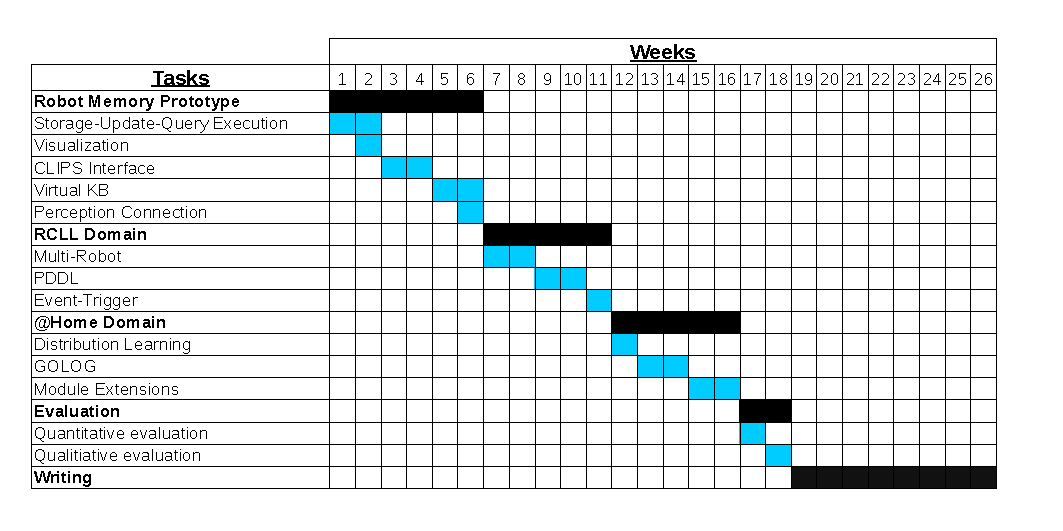
\includegraphics[width=\textwidth]{gantt-chart}%
  \vspace{-5mm}
  \caption{Gantt Chart of the thesis time schedule}
  \label{tab:gantt}
\end{table}
The time-schedule of the thesis is shown in \reftab{tab:gantt}. The
first part focuses on developing a robot-memory prototype with a CLIPS
interface and a virtual knowledge base. This prototype is then
iteratively improved to implement all other features needed in the
RCLL and in @Home. The robot-memory itself and both applications are
then evaluated and the rest of the time is spent on the written
thesis.


\bibliographystyle{plain}
\bibliography{../references}

\end{document}
